% !TEX encoding = UTF-8 Unicode

\documentclass[a4paper]{article}

\usepackage{color}
\usepackage{url}
\usepackage[utf8]{inputenc} % make weird characters work
\usepackage{graphicx}

\usepackage[serbian]{babel}
%\usepackage[english,serbianc]{babel} %ukljuciti babel sa ovim opcijama, umesto gornjim, ukoliko se koristi cirilica

\usepackage[unicode]{hyperref}
\hypersetup{colorlinks,citecolor=green,filecolor=green,linkcolor=blue,urlcolor=blue}

%\newtheorem{primer}{Пример}[section] %ćirilični primer
\newtheorem{primer}{Primer}[section]

\begin{document}

\title{Crveno-crna stabla\\ \small{Seminarski rad u okviru kursa\\Konstrukcija i analiza algoritama 2\\ Matematički fakultet}}

\author{Nikola Dimitrijević, 1086/2017\\ nikoladim95@gmail.com}
\maketitle

\abstract{
    Crveno-crna stabla su vrsta samobalansirajućih stabala. To je struktura podataka koja garantuje brze operacije umetanja, pretrage i brisanja.
    Svaki čvor stabla ima boju: crnu ili crvenu. Uz određena pravila i načine na koje se menja stablo dobija se gornja granica za koliko stablo može biti nebalansirano.

}

\tableofcontents

\newpage

\section{Osnovno}
\label{sec:uvod}
Crveno-crna stabla su struktura podataka koja omogućava brze operacije umetanja, brisanja i pretrage. Spadaju u samobalansirajuća stabala.
Svaki čvor ima dodatan bit (ili već neki tip podatka) koji reprezentuje boju čvora. Za baš crvenu i crnu boju su se autori odlučili pošto je pored pored klasične crne,
crvena boja najbolje iygledala na tadašnjim laserskim štampačima. Još jedan razlog je što su imali crvene i crne hemijske pa su tako crtali ova stabla.

\begin{figure}[h!]
\begin{center}
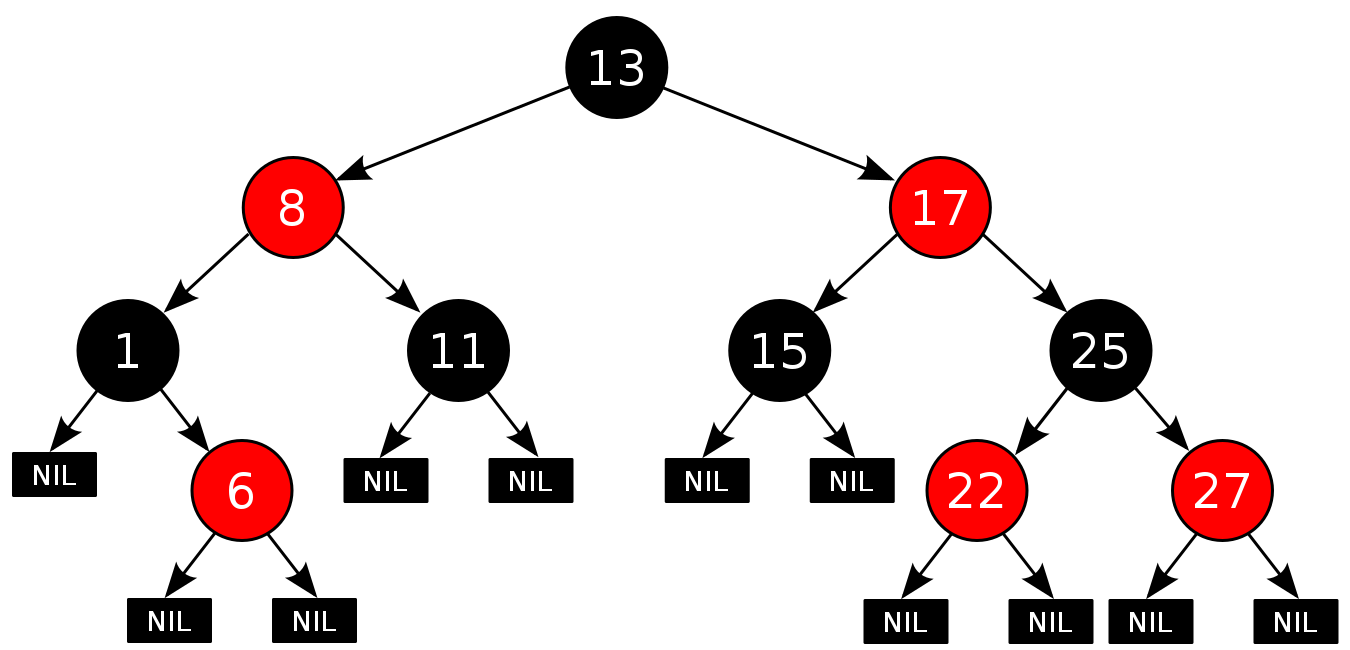
\includegraphics[scale=0.2]{example.png}
\end{center}
\caption{Primer crveno-crnog stabla}
\label{fig:primer}
\end{figure}

Za razliku od mnogih stabala, u implementacijama crveno-crnih stabala se umesto uobičajenih null pokazivača koriste specijalni null čvorovi (Na slici \ref{fig:primer} su označeni sa NIL) koji ne sadrže nikakve podatke
koji se unose u strukturu. Iako bi bilo moguće implementirati sve operacije crveno-crnih stabala korišćenjem običnih null pokazivača, ovako se uprošćavaju njihove implementacije.
Da bi se uštedelo na memoriji, umesto da postoji mnogo različitih null čvorova, moguće je imati jedan takav čvor u memoriji, a da svi ostali koji žele da pokazuju na null čvor pokazuju
baš na samo tog jednog.

Crveno-crna stabla se koriste za skladištenje podataka koji imaju uređenost, pošto se na osnovu poretka određuje pozicija elemenata u stablu.
\section{Svojstva}
\label{sec:termini_i_citiranje}

\begin{itemize}
        \item Svaki čvor je ili crn ili crven.
        \item Koren je crn.
        \item Svi listovi su crni.
        \item Ako je čvor crven, onda su mu oba sina crna.
        \item Svaki put od korena do svih NIL listova ima isti broj crnih čvorova.
\end{itemize}

\textit{Crna dubina} stabla je broj crnih čvorova od korena do listova, koji je za svaki put od korena do lista isti.

\section{Upoređivanje sa AVL stablima}
    Crveno-crna stabla su, kao i AVL stabla, samobalansirajuća. Oba pružaju O(log n) vreme pretrage, umetanja i brisanja.

    Razlika je u tome što crveno-crna stabla garantuju O(1) rotacija po operaciji umetanja. 
    Ta stvar zaista utiče na performanse u pravim implementacijama.


Reference koje se koriste u ovom tekstu zadate su u datoteci {\em seminarski.bib}. Prevođenje u pdf format u Linux okruženju može se uraditi na sledeći način:
\begin{verbatim}
pdflatex TemaImePrezime.tex 
bibtex TemaImePrezime.aux 
pdflatex TemaImePrezime.tex 
pdflatex TemaImePrezime.tex 
\end{verbatim}
Prvo latexovanje je neophodno da bi se generisao {\em .aux} fajl. {\em bibtex} proizvodi odgovarajući {\em .bbl} fajl koji se koristi za generisanje literature. 
Potrebna su dva prolaza (dva puta pdflatex) da bi se reference ubacile u tekst (tj da ne bi ostali znakovi pitanja umesto referenci). Dodavanjem novih referenci potrebno je ponoviti ceo postupak.  


Broj naslova i podnaslova je proizvoljan. Neophodni su samo Uvod i Zaključak. Na poglavlja unutar teksta referisati se po potrebi. 
\begin{primer}
U odeljku \ref{sec:naslov1} precizirani su osnovni pojmovi, dok su zaključci dati u odeljku \ref{sec:zakljucak}.
\end{primer}




\section{Slike i tabele}
\label{slike_i_tabele}

Slike i tabele treba da budu u svom okruženju, sa odgovarajućim naslo\-vima, obeležene labelom da koje omogućava referenciranje. 

\begin{primer} Ovako se ubacuje slika. Obratiti pažnju da je dodato i 
\begin{verbatim}
\usepackage{graphicx}
\end{verbatim}

%\begin{figure}[h!]
%\begin{center}
%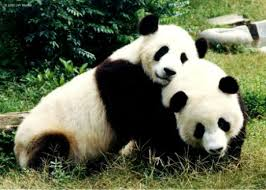
\includegraphics[scale=0.75]{pande.jpg}
%\end{center}
%\caption{Pande}
%\label{fig:pande}
%\end{figure}

%Na svaku sliku neophodno je referisati se negde u tekstu. Na primer, na slici \ref{fig:pande} prikazane su pande. 
\end{primer}

\begin{primer} I tabele treba da budu u svom okruženju, i na njih je neopho\-dno referisati se u tekstu. Na primer, u tabeli \ref{tab:tabela1} su prikazana različita pora\-vnanja u tabelama.

\begin{table}[h!]
\begin{center}
\caption{Razlčita poravnanja u okviru iste tabele ne treba koristiti jer su nepregledna.}
\begin{tabular}{|c|l|r|} \hline
centralno poravnanje& levo poravnanje& desno poravnanje\\ \hline
a &b&c\\ \hline
d &e&f\\ \hline
\end{tabular}
\label{tab:tabela1}
\end{center}
\end{table}

\end{primer}





\section{Prvi naslov}
\label{sec:naslov1}


Ovde pišem tekst. 
Ovde pišem tekst. 
Ovde pišem tekst. 
Ovde pišem tekst. 
Ovde pišem tekst. 
Ovde pišem tekst. 
Ovde pišem tekst. 
Ovde pišem tekst. 


\subsection{Prvi podnaslov}
\label{subsec:podnaslov1}

Ovde pišem tekst. 
Ovde pišem tekst. 
Ovde pišem tekst. 
Ovde pišem tekst. 
Ovde pišem tekst. 
Ovde pišem tekst. 
Ovde pišem tekst. 

\subsection{Drugi podnaslov}
\label{subsec:podnaslov2}

Ovde pišem tekst. 
Ovde pišem tekst. 
Ovde pišem tekst. 
Ovde pišem tekst. 
Ovde pišem tekst. 
Ovde pišem tekst. 

\section{Drugi naslov}
\label{sec:naslov2}

Ovde pišem tekst. 
Ovde pišem tekst. 
Ovde pišem tekst. 
Ovde pišem tekst. 

\subsection{... podnaslov}
\label{subsec:podnaslovN}

Ovde pišem tekst. 
Ovde pišem tekst. 
Ovde pišem tekst. 
Ovde pišem tekst. 
Ovde pišem tekst. 
Ovde pišem tekst. 

\section{n-ti naslov}
\label{sec:naslovN}

Ovde pišem tekst. 
Ovde pišem tekst. 
Ovde pišem tekst. 
Ovde pišem tekst. 
Ovde pišem tekst. 

\subsection{... podnaslov}
\label{subsec:podnaslovK}

Ovde pišem tekst. 
Ovde pišem tekst. 
Ovde pišem tekst. 
Ovde pišem tekst. 
Ovde pišem tekst. 

\subsection{... podnaslov}
\label{subsec:podnaslovM}

Ovde pišem tekst. 
Ovde pišem tekst. 
Ovde pišem tekst. 
Ovde pišem tekst. 
Ovde pišem tekst. 

\section{Poslednji naslov}
\label{sec:naslovM}

Ovde pišem tekst. 
Ovde pišem tekst. 
Ovde pišem tekst. 
Ovde pišem tekst. 
Ovde pišem tekst. 
Ovde pišem tekst. 
Ovde pišem tekst. 
Ovde pišem tekst. 
Ovde pišem tekst. 

\section{Zaključak}
\label{sec:zakljucak}

Ovde pišem zaključak. 
Ovde pišem zaključak. 
Ovde pišem zaključak. 
Ovde pišem zaključak. 
Ovde pišem zaključak. 
Ovde pišem zaključak. 
Ovde pišem zaključak. 
Ovde pišem zaključak. 
Ovde pišem zaključak. 
Ovde pišem zaključak. 
Ovde pišem zaključak. 
Ovde pišem zaključak. 


\addcontentsline{toc}{section}{Literatura}
\appendix
\bibliography{seminarski} 
\bibliographystyle{plain}

\appendix
\section{Dodatak}
Ovde pišem dodatne stvari, ukoliko za time ima potrebe.
Ovde pišem dodatne stvari, ukoliko za time ima potrebe.
Ovde pišem dodatne stvari, ukoliko za time ima potrebe.
Ovde pišem dodatne stvari, ukoliko za time ima potrebe.
Ovde pišem dodatne stvari, ukoliko za time ima potrebe.


\end{document}
